\chapter[Modelagem de Processos]{Modelagem de Processos}

\section{Introdução} \index{Introdução}

Este trabalho é continuação do trabalho “Uso do mapeamento de processos para o entendimento e identificação de melhorias no processo de desenvolvimento da FS Desenvolvimento de Soluções de Software” no qual foram mapeados, os problemas inerentes ao processo de desenvolvimento de software da empresa FS, bem como o próprio processo em si. A partir das conclusões tiradas da análise do processo atual da organização (As-Is), foi proposto um novo processo de desenvolvimento melhorado (To-Be) para solucionar alguns dos problemas levantados anteriormente.

Como surgiram vários processos e atividades novos no processo To-Be, foi priorizado apenas um processo para ser automatizado que foi: Processo de Registro de Problemas e Soluções, então a partir do novo processo de negócio, foi criado um terceiro processo de negócio que apresenta o uso de uma solução de software para automatizar uma parte do processo. Usando a ferramenta Bizagi Studio, foi criada a solução de software a partir do processo selecionado para automatização para resolver o problema de perda de informações e histórico de soluções dadas pelos integrantes da equipe.

A Seção 2 deste documento é um referencial teórico para auxiliar no entendimento dos conceitos relacionados à Gestão do Conhecimento (GC) que foram usados neste trabalho para resolver os problemas levantados no trabalho 1. A Seção 3 apresenta os pontos de melhorias identificados no processo atual, que foram resolvidos com ações e políticas ligados à GC. Na Seção 4, foram criados metas e indicadores para avaliar os impactos que as alterações poderiam ter no processo da empresa. Na Seção 5, foi realizada uma comparação entre o processo As-Is e o processo To-Be, para saber como o processo seria impactado com as alterações feitas. Na Seção 6, é descrita a solução de software criada com o Bizagi Studio e na Seção 7 foi feito um relato de experiência pessoal dos autores desse trabalho sobre a disciplina cursada e outros pontos relativos ao trabalho realizado.

\section{Fundamentação Teórica}\index{Fundamentação Teórica}
\subsection{Gestão do Conhecimento}\index{Gestão do Conhecimento}
No contexto atual de mercado, a crescente competição entre organizações exige que elas sejam capazes de desenvolver e gerenciar eficazmente seus recursos, quer sejam financeiros, estruturais ou de recursos humanos para se manterem competitivas. Dentro das organizações inseridas num contexto de rápido ritmo de circulação de informações, surgem muitas inovações  relacionadas com os mais diversos contextos, como por exemplo, no desenvolvimento ou venda de um produto ou serviço, nos métodos de produção, na abertura de novos negócios, ou ainda em reestruturação organizacional.  Desta forma, o conhecimento e o capital intelectual se tornaram fatores determinantes no sucesso das organizações e recursos estratégicos que são fonte de vantagem competitiva entre elas.  

Alguns autores que já dissertaram sobre o assunto, afirmam que vivemos hoje na sociedade do conhecimento, onde os meios de produção não estão nas linhas de montagem e máquinas, mas sim na cabeça e nas mãos das pessoas \cite{nonaka}. O desempenho das empresas está associado à capacidade de gerar novos conhecimentos e usá-los no desenvolvimento de produtos e serviços inovadores. Por isso a importância de saber gerí-lo adequadamente.

Para isso, elas devem ser hábeis para transformar informação em conhecimento. \cite{davenport}

A gestão do conhecimento pode ser entendida como o conjunto de práticas que identificam, criam e monitoram as variáveis e o ambiente ideais para que o conhecimento seja gerado e disseminado dentro de uma organização \cite{nonaka}. 

Mas antes de entender essas práticas, é preciso entender o que são os termos: conhecimento, informação e dados.

O termo conhecimento não possui um significado único, mas pode ser entendido como a informação inserida em um contexto, que passou por um processo de interpretação e contextualização, e dessa forma é interiorizada e incorporada pelas pessoas inseridas naquele contexto. Sendo assim, o conhecimento é gerado a partir da informação por meio da aplicação de modelos mentais e processos de aprendizagem das pessoas e entre elas. O conhecimento é intrínseco ao ser humano, individualmente construído, podendo relacionar-se à ação das pessoas e associar-se à intuição, às crenças, à experiência e aos valores que essas pessoas constroem.

O conhecimento é dinâmico e aumenta quando compartilhado. Ele está relacionado à ação em um determinado contexto. Desta forma, verifica-se a importância de gerar crenças, compromissos, situações e interações apropriadas, para que as informações possam ser convertidas em conhecimento e circular pelas organizações e assim, influenciar julgamentos, comportamentos e atitudes. \cite{nonaka}.

Outros autores \cite{fleury} consideram que o conhecimento é o resultado das interações que ocorrem em um ambiente e é desenvolvido através do processo de aprendizagem.

O conhecimento utiliza a informação como insumo. Esta pode ser definida como “dados processados e contextualizados” e também como “um conjunto de dados selecionados e agrupados segundo um critério lógico para a consecução de um determinado objetivo” \cite{angeloni}.

Os dados, insumos para geração de informação, podem ser definidos como observações documentadas ou resultados de medição. A partir de um contexto real, eles são extraídos, e não passam necessariamente por algum tipo de filtro. Dados são reflexo real do que é observado, e desta forma é assim documentado.

O conhecimento pode ser classificado em dois tipos: explícito e tácito \cite{nonaka}. O conhecimento explícito é tangível, visível, de natureza objetiva, de fácil comunicação e armazenamento, pode ser sistematizado em números e palavras, podendo ser facilmente comunicado e externalizado de diversas maneiras, como por exemplo, informações processadas, armazenadas e registradas (transmitidas) em livros e  manuais. Já o conhecimento tácito é subjetivo, “de difícil comunicação, transmissão e aprendizagem, oriundo de emoções, valores, ideais, intuição, habilidades e experiências pessoais.” \cite{nadai}. Este conhecimento está imbutido nas ações das pessoas, e em geral é desenvolvido e interiorizado pelo conhecedor.

A figura a seguir demonstra um metáfora acerca destes dois conhecimentos: o explícito representa o topo visível do iceberg; já o tácito, o que está por debaixo da imensidão das águas, é difícil de ser explicitado.

\begin{figure}[H]
\centering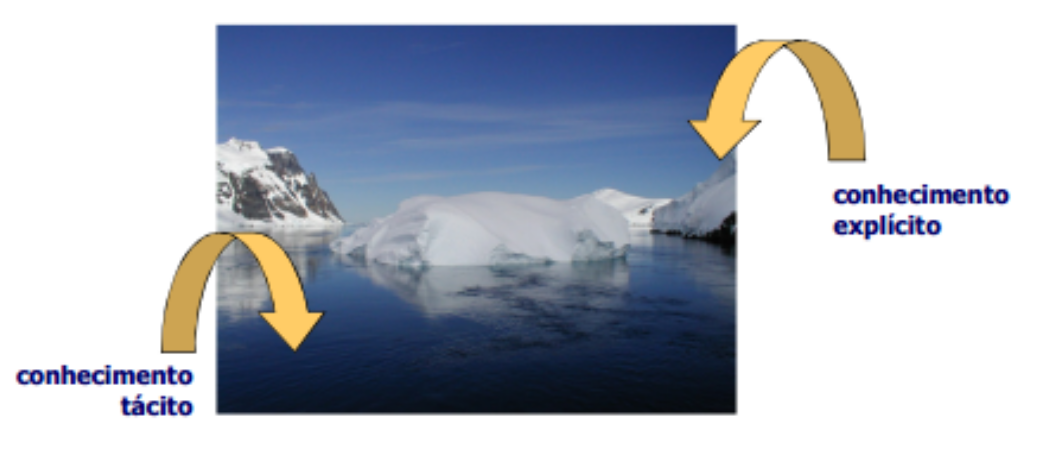
\includegraphics[scale=0.5]{figuras/tacitoExplicito.png}
\caption{\textit{Metáfora sobre os Conhecimentos}}
\end{figure}

Para esse conhecimento tácito realmente gerar valor para a empresa e vantagem competitiva, é necessário que ele seja convertido em conhecimento explícito.

Neste sentido, é mais importante às organizações gerirem as condições para a criação, o compartilhamento e a transferência deste tipo de conhecimento na organização, através de trabalho em equipe, do diálogo, entre outras práticas.

O processo de conversão  desse conhecimento, representado pela espiral do conhecimento, que compreende quatro etapas: Socialização, Externalização, Combinação e Internalização \cite{nonaka}. Ela está representada logo abaixo:

\begin{figure}[H]
\centering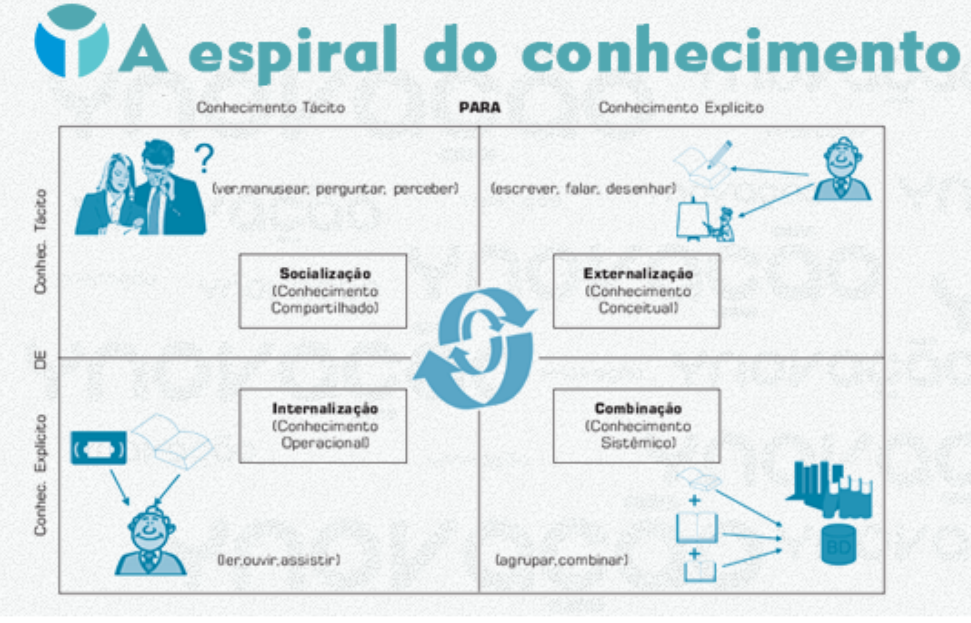
\includegraphics[scale=0.5]{figuras/espiralConhecimento.png}
\caption{\textit{Espiral do Conhecimento}}
\end{figure}

\begin{itemize}
\item \textbf{Socialização}: compartilhamento do conhecimento, ainda na forma tácita, por meio de experiências, criando novo conhecimento tácito (modelos mentais e habilidades técnicas) adquirido através de observação, prática ou imitação (sem necessariamente utilizar linguagem).  Exemplo: reuniões de braimstorm. 

\item \textbf{Externalização}: conhecimento tácito comunicado à terceiros (compartilhamento de conhecimento para as demais pessoas - essência da criação de conhecimento) utilizando analogias, representações e modelos, através de reflexão coletiva. Exemplo: mapas de conhecimento. 
Combinação: sistematizaçao e combinação de conhecimentos explícitos criando novos conhecimentos explícitos, registrando-os em documentos, banco de dados, etc. Exemplo: elaboração de um relatório com resumo de vendas, a partir de dados coletados em diversas áreas de uma empresa.
\item \textbf{Internalização}: incorporação de conhecimentos explícitos aos conhecimentos individuais das pessoas (conversão do conhecimento explícito para tácito). O conhecimento explícito uma vez disseminado, é convertido em tácito através de sua representação oral ou gráfica, criando novos modelos mentais e know-how. 
\end{itemize}

\section{Identificação e Realização de Melhorias}\index{Identificação e Realização de Melhorias}
No processo atual da organização (As-Is), foram encontrados pontos de melhorias. Esses pontos de melhorias foram distribuídos nas quatro fases da Gestão do Conhecimento. Para cada fase, foram definidas algumas práticas e políticas. Práticas são atividades ou métodos que facilitam o processo de GC e a transferência do conhecimento em pontos específicos do processo. Políticas são ações contínuas que devem ser executadas no dia-a-dia por todos da empresa  para complementar a GC e a transferência de conhecimento entre os integrantes da equipe.

\subsection{Socialização}\index{Socialização}
\subsubsection{Práticas}\index{Práticas}
\begin{itemize}
\item \textbf{Revisão em pares}: é uma técnica para realizar alguma atividade em dupla, de maneira que uma pessoa faz a atividade propriamente dita enquanto a outra permanece do lado vendo o que ela está fazendo. Desta forma, a segunda pessoa está atenta a erros de escrita e de lógica na execução da atividade, melhorando a qualidade e diminuindo a chance de retrabalho no futuro, Vale lembrar que é uma técnica que deve ser feita por meio de rodízios, ou seja, o esquema do pareamento deve ser invertido após algum tempo pré definido. Essa prática foi inserida nas atividades \textbf{Testar Requisitos}. No contexto de GC, a revisão em pares ajuda na obtenção do conhecimento por meio da observação, já que a segunda pessoa estará observando e aprendendo ao mesmo tempo que a primeira está fazendo as suas tarefas e por esse motivo, essa técnica foi adicionada à fase de Socialização da GC.
\item \textbf{Condução de workshops e treinamentos}: foram adicionadas novas atividades para condução de treinamentos em novos conhecimentos, caso seja necessário, e workshops para apresentação dos conhecimentos adquiridos durante a sprint. Essas atividades permitem que várias pessoas aprendam conhecimentos novos por meio da observação e por isso está encaixada na fase de Socialização, no entanto, também se encaixa na fase de Externalização, já que permite que uma pessoa transmita utilizando representações - apresentação de slides e registro escrito do conteúdo do treinamento, por exemplo - o seu conhecimento tácito para um grupo de uma maneira mais formal, já convertido em conhecimento explícito.
\end{itemize}

\subsubsection{Políticas}\index{Políticas}
\begin{itemize}
\item \textbf{Desenvolvimento em pares}: o desenvolvimento em pares, conhecido como pareamento, é uma técnica parecida com a revisão em pares, porém aplicada ao desenvolvimento de artefatos e não revisão de artefatos. Da mesma forma que a revisão em pares busca qualidade e menos retrabalho, o desenvolvimento em pares também, porém na hora de criar o artefato e não ao final do desenvolvimento do mesmo. Pelo fato de poder ser aplicada ao desenvolvimento de todo tipo de artefato, ela foi definida como uma política para ser executada no dia-a-dia em todos as atividades. Essa técnica permite, da mesma forma que a revisão em pares, o aprendizado pela observação e por isso também se encontra na fase de Socialização.
\item \textbf{Encontros diários}: são um forma de manter todos da equipe atualizados sobre tudo que está sendo feito, o que não foi feito até o momento e o porque de não ter sido feito de uma forma rápida e prática de maneira que não atrapalhe no desenvolvimento das atividades de cada um. Como permite a todos o compartilhamento de suas experiências diárias sobre o que estão realizando ou não, dificuldades que estão tendo, recursos e métodos que estão utilizando para atingir seus objetivos definidos, criam novos conhecimentos tácitos (modelos mentais e habilidades) para os demais participantes dos encontros. Por isso está na fase da Socialização. Mas também se encaixa na fase de Externalização, onde o conhecimento tácito das pessoas é articulado e transmitido a outros indivíduos (convertido em explícito).
\item \textbf{Rotação do trabalho}: a rotação do trabalho é uma política pensada para uniformizar o conhecimento dos integrantes da equipe nas mais diversas atividades do processo de desenvolvimento de software. Uma pessoa que um dia está realizando uma atividade de desenvolvimento, no outro pode realizar uma atividade de teste e depois uma atividade de requisitos. Sendo assim, sempre que ela muda de atividade, estará aprendendo coisas novas por meio da experiência e observação. Desta forma o conhecimento tácito é convertido em novo conhecimento tácito, construindo novos modelos mentais e habilidades, por isso está na fase de Socialização. 
\end{itemize}

\subsection{Externalização}\index{Externalização}
\subsubsection{Práticas}\index{Práticas}
\begin{itemize}
\item \textbf{Especificação de Requisitos}:  nesta atividade do processo o cliente pode externalizar o que precisa e quais são as suas vontades, desta forma encontra-se na fase de Externalização, quando o conhecimento é passado ao grupo por meio de uma reunião ou conversa informal. Mas também se encaixa na Combinação, já que as informações, desejos e necessidades transmitidas pelo cliente para elicitar requisitos do sistema são registrados em algum documento ou artefato. 
\end{itemize}

\subsubsection{Políticas}\index{Políticas}
\begin{itemize}
\item \textbf{Registro de informações de acompanhamento (Registro de trabalho)}: trata-se de uma política pensada para distribuir o conhecimento do que está e não está sendo feito. Dessa forma todos sempre poderão saber o que todos estão fazendo facilitando na comunicação e reduzindo o stress na hora de prestar contas do andamento do trabalho. Encontra-se na fase de Exernalização pelo fato de ser um conhecimento passado ao grupo na forma de conversa ou em uma reunião stand-up onde cada irá externalizar o conhecimento que adquiriu no dia e registrá-lo.
\end{itemize}

\subsection{Combinação}\index{Combinação}
\subsubsection{Práticas}\index{Práticas}
\begin{itemize}
\item \textbf{Construção de modelo de dados}: trata-se de uma prática inserida na atividade de mesmo nome que tem como objetivo o desenvolvimento de diagramas, esboços e modelos para auxiliar na construção de soluções de sistemas, antes de iniciar a codificação. Isso permite o registro de soluções e modelos que são desenvolvidos para um dado sistema, de forma a possibilitar que os envolvidos no projeto possam ter acesso a eles, reduzindo incoerências e discordâncias, e unificando a visão da solução para todos os integrantes. No contexto de GC, essa prática permite que o conhecimento explicíto seja padronizado e registrado para visualização de todos, por isso está encaixada na fase Combinação. Esta prática também está associada também à Externalização, pois o conhecimento precisa ser externalizado e comunicado às pessoas, pde ara  ser registrado em seguida.
\item \textbf{Criação de Relatório Gerencial}: trata-se de uma prática inserida na atividade de Gerar Relatório Gerencial e diz respeito à elaboração de um documento para o cliente, ao final de cada iteração, onde consta o parecer do gerente em relação aos aspectos do desenvolvimento do projeto, incluindo fatos e acontecimentos positivos e negativos relevantes sobre ele. Esta tarefa é atribuição do Gerente de Projeto, que usa como base o registro de trabalho dos funcionários; isso reduz o stress e sobrecarga sobre ele. No contexto de GC, o registro desses fatos e acontecimentos configura essa prática dentro de Combinação, pois é um momento onde vários conhecimentos são registrados formalmente para poderem, posteriormente, serem internalizados. 
\item \textbf{Geração de documentação automática (Ex.: PHPDoc, JavaDoc, etc)}: esta prática se refere à geração de documentação automática a partir do código, quando iniciar a atividade de implementação em um dado projeto. Isto auxilia os desenvolvedores quando for necessário introduzir e manipular comentários em trechos do código de uma forma eficiente para facilitar a reutilização futura desses comentários, que representam fonte geradora de conhecimentos acerca do código. Por isso, esta prática está inserida na Combinação, a documentação de código é gerada a partir do código implementado, os conhecimentos explícitos referentes ao código existente são combinados para gerar novos conhecimentos explícitos, a documentação.
\item \textbf{Criação de padronização de Código fonte (documento de estilo e design)}: é uma prática para tornar o código fonte das aplicações produzidas mais legível para todos, desde o integrante novo até o testador e mantenedor. Com um documento de padronização, os conhecimentos sobre boas práticas de desenvolvimento podem ser reunidos para tornar as atividades de desenvolvimento e manutenção mais simples e práticas. Pelo fato de haver um documento que reúna vários conhecimentos e informações que foram padronizados baseado em padrões de estilo e design já existentes, encontra-se na fase de Combinação. 
\item \textbf{Geração de Relatório de Acompanhamento do Portfólio}: trata-se de uma tarefa dentro da atividade Supervisionar Manutenção do Portfolio na qual todo o conhecimento que se tem sobre o uso do portfolio é combinado em um relatório a ser apresentado para a gerência de alto nível, escrito a partir dos registros realizados nele, acerca do uso e os impactos que o portfolio tem causado na execução das atividades diárias de cada um. Por esse motivo, encontra-se na fase de Combinação.
\end{itemize}

\subsubsection{Políticas}\index{Políticas}
\begin{itemize}
\item \textbf{Uso do portfólio tecnológico}: o uso do portfolio é uma política pensada para criar e manter uma consciência coletiva da necessidade de usar o portfolio para manter registros dos problemas, soluções e conhecimentos e tudo o que é produzido na empresa. Por ser um local de reunião de conhecimentos formalmente registrados encontra-se na fase de Combinação.
\end{itemize}

\subsection{Internalização}\index{Internalização}

\subsubsection{Políticas}\index{Políticas}
\begin{itemize}
\item \textbf{Consulta à documentação}: o uso da documentação nada mais é do que a consulta à documentação associada ao projeto para assimilar os conhecimentos que foram combinados para gerá-la. No contexto da GC, foi definida na fase de Internalização, pois a leitura do material produzido é uma forma de aprendizado transformando o conhecimento explícito, que foi combinado para a criação da documentação, em tácito, que é o conhecimento pessoal.
\item \textbf{Consulta ao portfólio tecnológico}: da mesma forma que a consulta à documentação, a consulta ao portfolio também é para assimilar conhecimentos explícitos que foram combinados para criar o portfolio e dessa maneira transformá-lo em conhecimento tácito, por isso encontra-se na fase de Internalização.
\item \textbf{Codificação}: é a atividade de programar a solução de software a ser desenvolvida. É o momento onde o desenvolvedor “aprende fazendo” após ter incorporado uma série de conhecimentos, por isso o conhecimento explícito é convertido para tácito por meio do código e por isso encontra-se na fase de Internalização.
\end{itemize}

\subsection{Portfólio Tecnológico}\index{Portfólio Tecnológico}
Para solucionar o problema de perda de conhecimento e de soluções foi idealizado uma espécie de repositório de conhecimento no qual todos os integrantes da FS pudessem registrar problemas que tiveram durante a execução de suas atividades assim como as soluções dadas por outros colegas de trabalho. Esses problemas estariam associados a determinadas tecnologias, as quais estariam descritas em um portfolio tecnológico.

O portfolio tecnológico consiste em um acervo no qual seriam guardadas as descrições de tecnologias já usadas e em uso nos projetos da empresa. Por meio do portfolio seria possível registrar e compartilhar boas práticas, lições aprendidas, recomendações de uso, além de outras informações relevantes a respeito da tecnologia, além de poder deixar registrado quem dentro da empresa domina determinada tecnologia. Um exemplo de estrutura da disposição das informações no portfolio é encontrado no Apêndice A. Junto à criação de um portfolio tecnológico, surge a necessidade da criação de um novo papel na empresa, o qual denominamos Gestor do Conhecimento. Ele seria responsável por mapear as tecnologias em uso, supervisionar a manutenção do portfolio e verificá-lo quanto à sua consistência.

Alguns pontos de automatização foram identificados no processo melhorado (To-Be). Esses pontos são o Registro diário do trabalho, Registro de problemas e soluções e Portifólio tecnológico. Nesses pontos específicos, caberiam soluções de software para auxiliar no controle da execução do processo da empresa, no entanto, foi priorizado junto ao cliente apenas o Registro de problemas e soluções, que é uma parte do portfolio tecnológico.

\section{Metas e Indicadores}\index{Metas e Indicadores}
De acordo com Rua (2004), “indicadores são medidas que representam ou quantificam um insumo, um resultado, uma característica ou o desempenho de um processo, de um serviço, de um produto ou da organização como um todo“. Segundo Costa (2007), “metas são valores quantitativos ou qualitativos a serem atingidos em certo momento futuro preestabelecido”.
Com o intuito de analisar os resultados da alteração do processo de desenvolvimento não paralelo e tendo como base os principais problemas do processo, foram definidos metas e  indicadores, apresentados nas subseções a seguir.

\subsection{Metas}\index{Metas}
\begin{itemize}
\item Mapear, no mínimo, 80\% das tecnologias utilizadas na empresa e registrá-las no portfólio tecnológico até março/2015;
\item Assegurar que, até março de 2015, todos os funcionários estejam registrando diariamente as atividades que estão sendo executadas;
\item Alcançar, no mínimo, 80\% de participação dos funcionários no repositório do conhecimento até julho/2015;
\item Assegurar que todos os funcionários tenham, em um ano, ao menos uma contribuição por sprint para o repositório do conhecimento.
\end{itemize}

\subsection{Indicadores}\index{Indicadores}

\subsubsection{Indicadores com foco nos recursos humanos}\index{Indicadores com foco nos recursos humanos}
\begin{table}[H]
\caption{Índice de Absenteísmo.}
\centering
\begin{tabular}{ | p{3cm} | p{9cm}| }
\hline
\textbf{Indicador: 01} & Índice de Absenteísmo.\\ \hline
\textbf{O quê mede} & Percentual de abstenções dos funcionários. \\ \hline
\textbf{Quem mede} & Responsável pelo RH. \\ \hline
\textbf{Quando medir} & Mensalmente. \\ \hline
\textbf{Por quê medir} & Dar um indicativo do nível de satisfação dos funcionários, por meio da análise das faltas ao trabalho. \\ \hline
\textbf{Como medir} & 
\begin{center}
\begin{equation}
\frac{Horas Liquidas faltantes}{Horas Liquidas Disponíveis}*100
\end{equation}
\end{center}
Onde,
Horas líquidas faltantes – total de horas faltantes, exceto férias, horas de treinamento e licenças maternidade e de saúde acima de 15 dias.
Horas líquidas disponíveis – total de horas brutas (jornada contratual), exceto o repouso remunerado.
 \\ \hline
\textbf{Situação atual} & - \\ \hline
\textbf{META} & jan/2015 - 5,00\% ; fev/2015 - 3,00\% \\ \hline
\end{tabular}
\end{table}

\begin{table}[H]
\caption{Índice de Treinamento.}
\centering
\begin{tabular}{ | p{3cm} | p{9cm}| }
\hline
\textbf{Indicador: 02} & Índice de Treinamento.\\ \hline
\textbf{O quê mede} & Coeficiente de horas de treinamento por funcionário. \\ \hline
\textbf{Quem mede} & Gerente do conhecimento. \\ \hline
\textbf{Quando medir} & Semestralmente. \\ \hline
\textbf{Por quê medir} & Obter o nível de investimento da empresa no desenvolvimento dos recursos humanos. \\ \hline
\textbf{Como medir} & 
\begin{center}
\begin{equation}
\frac{Total de Horas de Treinamento}{Número de Funcionários}
\end{equation}
\end{center}
Onde,
Total de horas de treinamento  – horas de treinamento dos funcionários no período analisado.
Número de funcionários – número de funcionários ativos na empresa.
 \\ \hline
\textbf{Situação atual} & 0 horas \\ \hline
\textbf{META} & jul/2015 - 08 horas ; jan/2016 - 12 horas  \\ \hline
\end{tabular}
\end{table}

\subsubsection{Indicador com foco nos clientes}\index{Indicador com foco nos clientes}

\begin{table}[H]
\caption{Índice de Satisfação dos Clientes.}
\centering
\begin{tabular}{ | p{3cm} | p{9cm}| }
\hline
\textbf{Indicador: 02} & Índice de Satisfação dos Clientes.\\ \hline
\textbf{O quê mede} & Satisfação dos clientes da empresa. \\ \hline
\textbf{Quem mede} & Gerente de Projeto. \\ \hline
\textbf{Quando medir} & Ao final de cada sprint dos projetos. \\ \hline
\textbf{Por quê medir} & Obter o grau de satisfação dos clientes, por meio da aplicação de questionários. \\ \hline
\textbf{Como medir} & Aplicar um questionário online de satisfação aos clientes. As questões devem ser compostas por uma escala de likert de 5 pontos. Realizar uma média ponderada para obtenção de um valor entre 1 e 5.
O questionário, criado com base no “Modelo de Satisfação de Clientes” do site SurveyMonkey, é presentado no apêndice B. \\ \hline
\textbf{Situação atual} & - \\ \hline
\textbf{META} & Ao final de cada projeto, obter um grau de satisfação entre 4 e 5. \\ \hline
\end{tabular}
\end{table}

\section{Simulação e comparações As-Is x To-Be}\index{Simulação e comparações As-Is x To-Be}
\textbf{Subprocesso priorizado para melhoria: Desenvolvimento não-paralelo.}

Este subprocesso compreende o desenvolvimento de uma solução de software, incluindo atividades de definição de requisitos, arquitetura, codificação e teste sendo executadas de forma sequencial. Ele está representado abaixo (AS-IS):

\begin{figure}[H]
\centering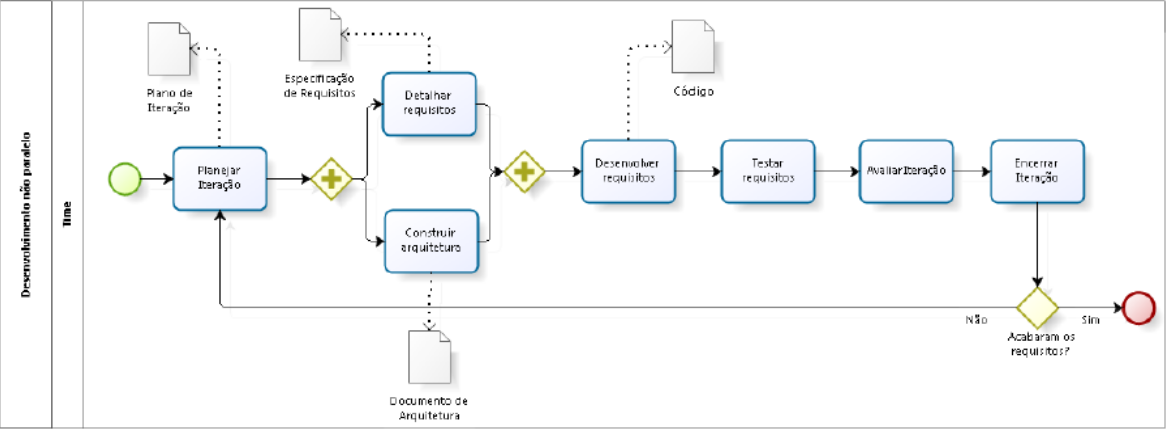
\includegraphics[scale=0.3]{figuras/asIs.png}
\caption{\textit{Versão 1.0 do subprocesso de Desenvolvimento não-paralelo.}}
\end{figure}

Juntamente com os outros subprocessos que fazem parte do Macro Processo de Desenvolvimento de Software, o subprocesso de Desenvolvimento Não-paralelo foi simulado para verificar seu comportamento no período de dois meses, iniciando 10 instâncias e considerando a execução das atividades de trabalho desde às oito da manhã e com duração de oito horas, repetindo-se diariamente de segunda a sexta-feira.

A seguir está a imagem do momento em que a simulação foi realizada, contendo os dados utilizados:

\begin{figure}[H]
\centering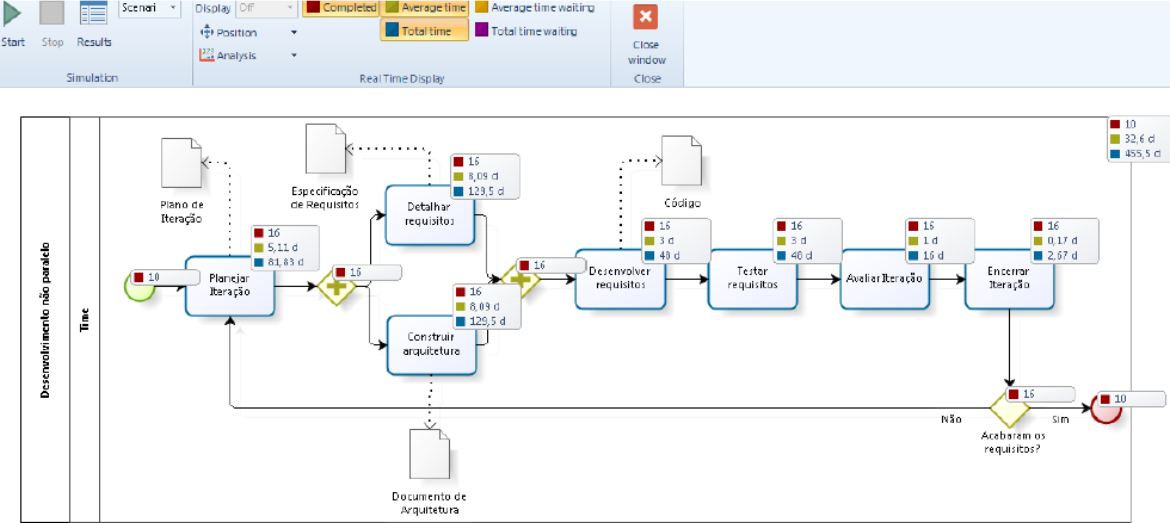
\includegraphics[scale=0.3]{figuras/simulacaoAsIs.png}
\caption{\textit{ Simulação do subprocesso de Desenvolvimento Não-paralelo (AS-IS).}}
\end{figure}

A simulação gerou como resultados os dados apresentados abaixo, relacionados a utilização dos recursos no subprocesso:

\begin{figure}[H]
\centering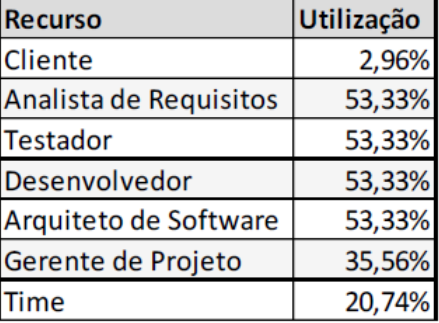
\includegraphics[scale=0.5]{figuras/participacaoPapeis.png}
\caption{\textit{Participação dos papeis no subprocesso.}}
\end{figure}

Fazendo uma análise a partir destes dados, observa-se que os recursos estão sendo  utilizados de forma equilibrada quando se trata dos papeis envolvidos dentro da equipe de projeto, excetuando o cliente, que possui uma participação bem reduzida neste subprocesso, participando de uma atividade apenas, a de Detalhamento dos Requisitos. 

Conclui-se que os recursos estão sendo bem aproveitados e bem utilizados neste subprocesso. A imagem abaixo, resultado da simulação também, apresenta outros dados de execução em tempo real do subrpocesso:

\begin{figure}[H]
\centering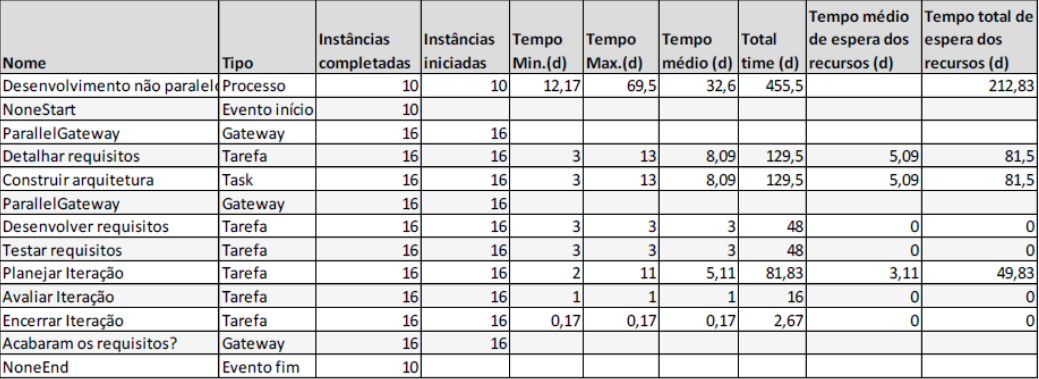
\includegraphics[scale=0.4]{figuras/resultadoSimulacao.png}
\caption{\textit{Resultado da simulação do subprocesso Desenvolvimento Não-paralelo.}}
\end{figure}

A análise de dados mostra que todas as instâncias iniciadas no subprocesso foram concluídas em tempo considerável, ou seja, o processo não apresenta problemas na execução das suas atividades. O tempo de espera para as atividades que ocorrem em paralelo (Detalhar requisitos e Construir arquitetura) é relativamente pequeno e não representa gargalo para o subprocesso. 

Percebe-se também que não há problemas relacionados à utilização e aproveitamento de recursos das atividades. 

Porém, de acordo com o contexto da empresa, existem alguns problemas associados a atividades não previstas no processo, que por sua vez, podem resultar em uma mudança na execução do fluxo, causando estresse na equipe, perda de informações e atrasos nos projetos.

Para solucionar e eliminar esses problemas, foram inseridas atividades relacionadas a acompanhamento de projeto, elaboração de relatórios, entre outras para apoiar a gestão do conhecimento dentro da empresa.

Tendo isso em vista, o processo foi remodelado e atividades foram inseridas. Na Figura a seguir, encontra-se a versão 2.0 do processo. 

\begin{figure}[H]
\centering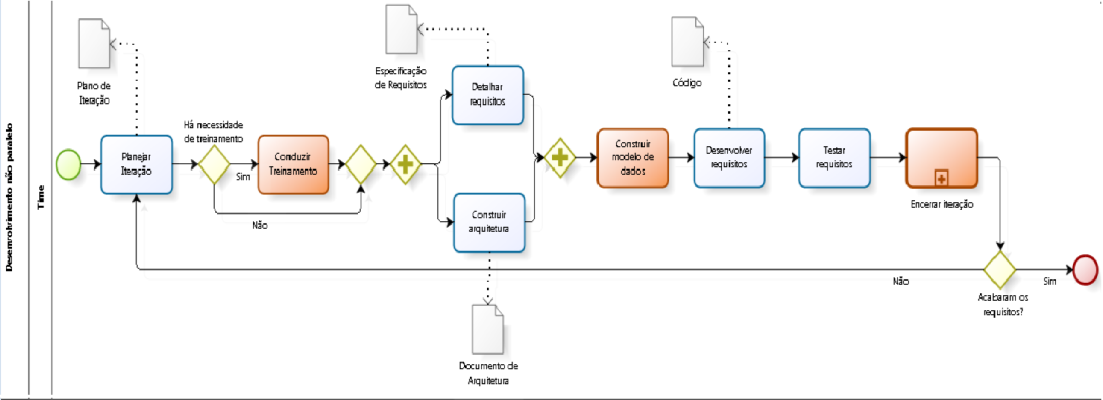
\includegraphics[scale=0.4]{figuras/subprocessoDevNaoParalelo2.png}
\caption{\textit{Versão 2.0 do subprocesso de Desenvolvimento Não-Paralelo.}}
\end{figure}

Neste processo, foram inseridas as seguintes atividades, destacadas na cor laranja: \textbf{Conduzir Treinamento} e \textbf{Construir Modelo de Dados}. As antigas atividades \textbf{Avaliar Iteração} e \textbf{Encerrar Iteração} foram substituídas pelo subprocesso de \textbf{Encerrar Iteração}, também destacado na cor laranja.

A atividade \textbf{Conduzir Treinamento} leva em consideração a necessidade de ministrar algum tipo de treinamento acerca de alguma tecnologia, feramenta, método, recurso ou algum conhecimento que será utilizado para o desenvolvimento de uma dada solução, possibilitando que o conhecimento seja compartilhado e uniformizado entre os integrantes da equipe e evitando atrasos e empecilhos durante o decorrer do projeto.

A atividade \textbf{Construir Modelo de Dados} trata do desenvolvimento dos esboços, modelos e diagramas de alto  baixo nível necessários para implementação do sistema, na sprint corrente, antes de iniciar a codificação. Isso permite o registro de soluções de modelagem que são dadas a um sistema, de forma que os envolvidos no projeto possam ter acesso, reduzindo as perdas e incoerências nas informações acerca de soluções de um dado projeto. Outra vantagem desta atividade, é que permite consulta de soluções de outros projetos , quando a equipe achar necessário pesquisar soluções.

O subprocesso \textbf{Encerrar Iteração} inclui as as atividades: \textbf{Gerar Relatório Gerencial}, \textbf{Avaliar Iteração}, \textbf{Conduzir Workshop} e \textbf{Apresentar Produto}, seu modelo é apresentado na Figura, a seguir.

\begin{figure}[H]
\centering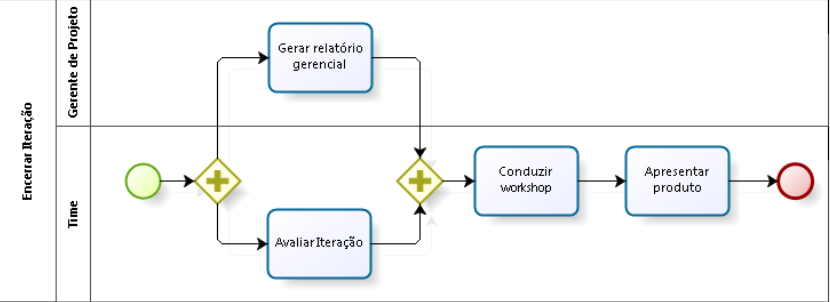
\includegraphics[scale=0.5]{figuras/encerrarIteracao.png}
\caption{\textit{Subprocesso Encerrar Iteração.}}
\end{figure}

A atividade \textbf{Gerar Relatório Gerencial} trata da elaboração de um documento para o cliente, ao final de cada iteração, onde consta o parecer do gerente em relação aos aspectos do desenvolvimento do projeto, incluindo fatos e acontecimentos positivos e negativos relevantes sobre ele. Esta tarefa é atribuição do Gerente de Projeto, que a realiza com base nos registros diários do trabalho dos funcionários, reduzindo seu stress e sobrecarga. 

A atividade \textbf{Avaliar Iteração} incorpora análise e retrospectiva da iteração do projeto. 

A atividade \textbf{Conduzir Workshop} visa trazer para toda a equipe envolvida no projeto, tudo o que foi aprendido e compartilhado em termos de conhecimento individual e em grupo adquirido durante o desenvolvimento do mesmo.

A atividade \textbf{Apresentar Produto} está relacionada a apresentação e entrega do produto (software) ao cliente final. 

Esta nova versão do processo foi simulada e os resultados encontram-se nas Figuras 7 e 8, a seguir.

\begin{figure}[H]
\centering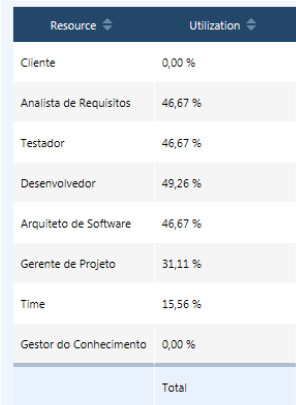
\includegraphics[scale=0.5]{figuras/utilizacaoRecursos.png}
\caption{\textit{Utilização dos Recursos.}}
\end{figure}

\begin{figure}[H]
\centering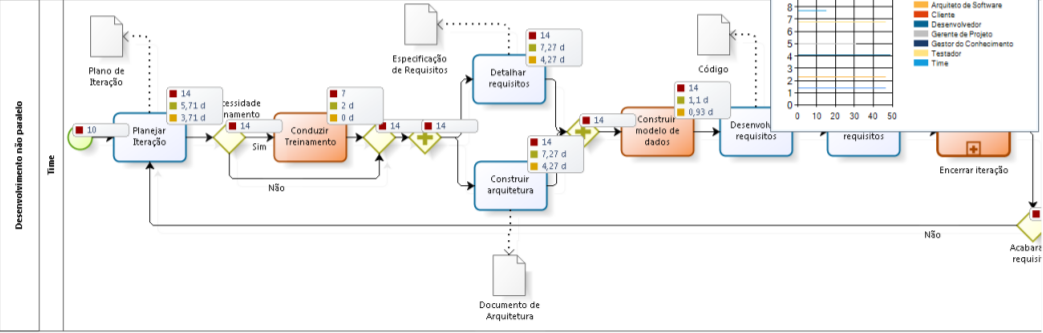
\includegraphics[scale=0.5]{figuras/simulacaoSubProcessoDevNaoParalelo.png}
\caption{\textit{Simulação do subprocesso Desenvolvimento não-paralelo (TO-BE).}}
\end{figure}

O subprocesso foi simulado para verificar qual seria o comportamento dele utilizando os mesmos parâmetros da simulação do primeiro subprocesso (período de dois meses, iniciando 10 instâncias e considerando a execução das atividades de trabalho desde às oito da manhã e com duração de oito horas, repetindo-se diariamente de segunda a sexta-feira).

De acordo com as imagens acima, percebe-se que os recursos estão sendo melhor utilizados e distribuídos no processo, com exceção do Cliente, que não possui participação nesse subprocesso, e do Gestor do conhecimento, cuja participação é mais efetiva em um outro subprocesso, o de \textbf{Gestão do conhecimento}, que foi criado para dar suporte ao processo de desenvolvimento de software, com objetivo de solucionar os problemas identificados no processo de desenvolvimento (Estresse da Equipe, Perda de Histórico e Perda de Soluções), pois eles estão estritamente relacionados com a gestão do conhecimento na empresa.

\begin{figure}[H]
\centering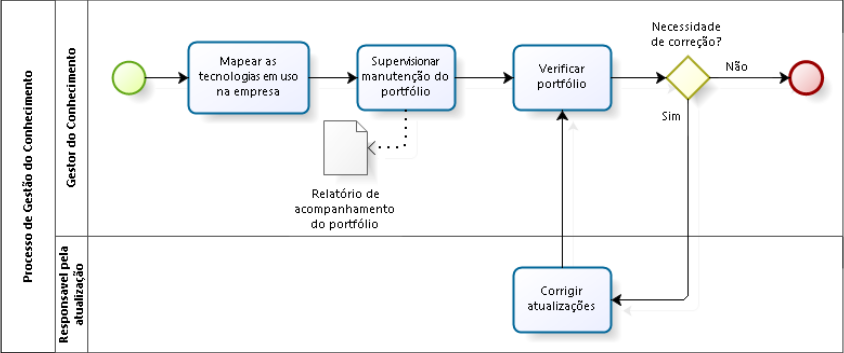
\includegraphics[scale=0.5]{figuras/subprocessoGC.png}
\caption{\textit{Subprocesso de Gestão do Conhecimento.}}
\end{figure}

Este subprocesso é composto pelas atividades: \textbf{Mapear as tecnologias em uso na empresa, Supervisionar Manutenção do portfólio, Verificar Portfólio e Corrigir atualizações}.

A atividade de \textbf{Mapear as tecnologias em uso na empresa} trata do mapeamento de todas as tecnologias já utilizadas ou em uso dentro do projetos da empresa. Isso é registrado em um portfólio. Desta forma, todo o conhecimento (tecnologias, experiências, etc) fica disponível para todos os funcionários dentro da empresa, eliminando o stress da equipe em ficar recuperando todo o conhecimento gerado dentro da empresa.

A atividade de \textbf{Supervisionar Manutenção do Portfólio} cuida da manutenção do que foi registrado no portfólio de projetos, gerando um relatório de acompanhamento do portfólio. Os conhecimentos armazenados precisam estar sempre atualizados com o fim de estarem sempre à disposição daqueles que precisarem no momento que precisarem. 

A atividade de \textbf{Verificar Portfólio} averigua a necessidade da realização de modificações no portfólio. Caso isso seja necessário, essas modificações precisam ser feitas, e isso é realizado na atividade de \textbf{Corrigir Atualizações}.

Após as alterações no processo de negócio da empresa com a adição de novos subprocessos, atividades e políticas, o macro processo da empresa teve algumas alterações. O subprocesso de \textbf{Gestão do Conhecimento} citado anteriormente, é executado em paralelo com todo o processo de desenvolvimento de software da empresa, assim como o subprocesso \textbf{Registro de Problemas e Soluções} para solucionar o problema de perda de informações e soluções dadas pelos integrantes. 

\begin{figure}[H]
\centering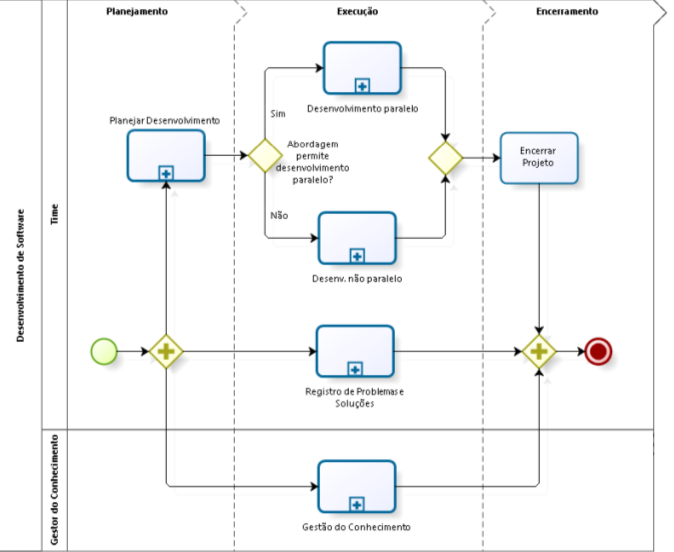
\includegraphics[scale=0.5]{figuras/imagemAleatoria.png}
\caption{\textit{Processo Completo de Desenvolvimento de Software.}}
\end{figure}

Além dos processos já citados, foi criado o processo \textbf{Registro de Problemas e Soluções} que visa auxiliar no controle de soluções dadas para os problemas que a equipe teve durante a execução de um projeto. Este subprocesso é composto de duas atividades em paralelo \textbf{Registrar problema} e \textbf{Registrar solução}. 

Na atividade \textbf{Registrar problema} o integrante da equipe pode registrar um problema que teve durante a execução de alguma atividade e, caso seja solicitado pelo Gestor do Conhecimento, realizar alguma alteração no problema que ele cadastrou por motivos de inconsistências.

Na atividade \textbf{Registrar soluções} um integrante poderia, caso soubesse, resolver um problema que outro integrante cadastrou e da mesma forma, caso solicitado pelo Gestor do Conhecimento, realizar alguma alteração na solução cadastrada se algo estiver inconsistente.

\begin{figure}[H]
\centering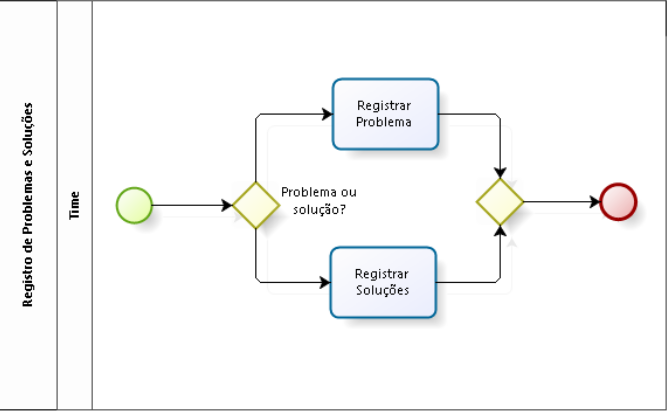
\includegraphics[scale=0.5]{figuras/processoDoBizagi.png}
\caption{\textit{Processo de Registro de Problemas e Soluções.}}
\end{figure}

\section{Solução: Repositório do Conhecimento}\index{Solução: Repositório do Conhecimento}
A solução criada para resolver o problema de perda de conhecimento foi chamada de Repositório de Conhecimento. É uma solução de software criada a partir da ferramenta Bizagi Studio que visa automatizar esta pequena parte do processo de negócio da empresa para solucionar o problema especificado. 

Na solução é possível cadastrar e pesquisar problemas e soluções dadas pelos integrantes da equipe. Foi feita uma análise prévia de requisitos na qual muitos requisitos foram levantados junto ao cliente, no entanto, por motivos de tempo, somente algumas features foram priorizadas. 

As features priorizadas podem ser vistas no Capítulo XX deste documento, onde encontra-se a rastreabilidade desde Temas de Investimento elicitados até as Histórias de Usuários detalhadas usando-se a técnica do 3C.

\section{Feedback da matéria}\index{Feedback da matéria}
Esta seção destina-se a fornecer um feedback pessoal dos autores deste trabalho sobre como foi a experiência vivida no decorrer do semestre na execução do trabalho e nas tarefas da disciplina. Tudo o que foi relatado nessa seção foi um consenso entre todos os membros da equipe de Modelagem de Processo, de maneira que todos concordam com que está escrito. 

\subsection{Relato de experiência}\index{Relato de experiência}
As disciplinas de Modelagem de Processos e Requisitos de Software da Universidade de Brasília - Gama, foram ministradas, pela primeira vez, em conjunto. No entanto, por ser a primeira vez que este esquema foi realizado, alguns erros ocorreram no decorrer do semestre, já que tanto o professor quantos os alunos, não sabiam ao certo o que esperar da matérias, dos trabalhos e da relação entre os grupos. Por exemplo, a interação que deveria ocorrer entre os grupos das duas matérias não ficou clara durante toda a execução do trabalho e com isso os grupos não sabiam o que fazer e qual a extensão das atividades de um grupo e de outro.

As aulas da disciplina de modelagem, que foram ministradas, foram muito proveitosas em relação ao conteúdo, já que o professor dominava o conteúdo e o explicava bem. No entanto, algumas aulas que estavam planejadas para serem ministradas, não foram por alguns imprevistos que ocorreram no decorrer do semestre como falta de água no campus e a semana universitária. Além disso, em algumas aulas não foi possível terminar o conteúdo por falta de tempo, mas não foram concluídas posteriormente, o que acabou deixando uma lacuna naqueles conteúdos, e mesmo assim ainda foram cobrados nos trabalhos como matérias dadas. 

Da forma como o trabalho foi conduzido este semestre o grupo de modelagem acabou fazendo o trabalho de requisitos novamente, no sentido de ter necessariamente que ajudar o grupo de requisitos e o grupo de requisitos não poder ajudar nas tarefas de modelagem. As relações de cliente e contratado também não ficaram claras, até porque esses relacionamentos mudaram ao longo do semestre o que contribuiu ainda mais para tornar as coisas confusas.

Não podemos esquecer de citar que cada integrante faz em média cinco matérias por semestre e disciplinas como Modelagem de Processo exigem muito mais tempo do que de fato cada integrante pode disponibilizar para a disciplina, o que acaba por forçar encontros em finais de semanas e feriados para compensar a falta de tempo. Uma resposta pragmática seria: Porque não pegar menos matérias? E uma resposta mais pragmática ainda seria: Porque não podemos! Temos que pegar pelo menos 24 créditos por semestre para nos formarmos, o que implica em pelo menos seis matérias por semestre, ou seja, já estamos pegando menos matérias do que precisamos!

\subsection{Interação entre a equipe de Modelagem de Processo}\index{Interação entre a equipe de Modelagem de Processo}
A equipe teve, durante a execução do primeiro trabalho, dois integrantes que já se conheciam e tinham um ótimo nível de relacionamento. Após a apresentação do primeiro trabalho, um grupo foi dissolvido e as pessoas foram realocadas em outros grupos, com isso, um novo integrante entrou no grupo de Modelagem de Processo. A integração entre os três integrantes foi também fácil,  tranquila e livre de atritos de qualquer tipo, já que os três trabalharam e colaboraram para o desenvolvimento do trabalho.

\subsection{Interação entre as equipes}\index{Interação entre as equipes}
As equipes das duas disciplinas tiveram no início um problema de comunicação com um dos integrantes do grupo de Requisitos de Software, o que rendeu um problema na execução das atividades do grupo de requisitos. No entanto, após uma conversa aberta com todos, o mal entendido foi resolvido entre todos e todos puderam contribuir para o andamento do trabalho. 

Pelo mesmo motivo do acréscimo de um integrante ao grupo de modelagem, um integrante entrou no grupo de requisitos após o primeiro trabalho. Mesmo com um integrante a mais, não houve problema algum durante a execução do segundo trabalho, já que todos se reuniram para fazer o que deviam sem problemas.

Na grande maioria das vezes os dois grupos estavam juntos para realizar as atividades, sinal da boa relação entre todos os integrantes das equipes, com isso, os grupos sempre estavam a par do que o outro grupo estava fazendo, ainda que essa percepção não tenha sido compartilhada pelo professor algumas vez.

\subsection{Sugestões de melhoria}\index{Sugestões de melhoria}
Como sugestão de melhoria para as duas matérias, é preciso definir melhor os papéis de cada grupo e até onde se estendem as responsabilidades de cada grupo, para que não ocorra o que aconteceu esse semestre e os grupos fiquem sem saber o que fazer e como fazer. Uma sugestão seria não ter prova já que o cancelamento da que teria nesse semestre foi muito oportuno para todos já que liberou mais tempo para realizar as atividades do trabalho e das outras disciplinas que cada integrantes faz na faculdade. 

O número de matérias que pegamos representa um número elevado de projetos e trabalhos para se preocupar no espaço de tempo de um semestre, então uma sugestão seria mudar datas de trabalhos para que não coincidam com datas de trabalhos e provas de outras matérias, ainda que signifique apresentar um pouco antes ou um pouco depois do período crítico do semestre.

\subsection{Lições aprendidas}\index{Lições aprendidas}
Concluímos que a universidade não condiz com a realidade do trabalho assalariado, visto que, em um projeto onde há várias pessoas envolvidas, se uma pessoa não faz o que deveria fazer, essa pessoa tem grandes chances de ser demitida ou rebaixada da sua posição atual, de maneira que cada pessoa por mais dificuldade que tenha deve correr atrás e não esperar que ajuda venha do céu. O problema não é ter dificuldades ou não entender algo, o problema é não fazer nada a respeito para mudar a situação.

Concluímos também que imprevistos sempre acontecem e devemos estar preparados para mudar os planos feitos para contorná-los. 

\subsection{Resumo geral}\index{Resumo geral}
A matéria foi muito boa em termos de conteúdo, porém foi um tanto densa e cansativa, o que acabou por minar a vontade e alegria de fazer o trabalho na reta final do mesmo o que gerou muito estresse na equipe e perda de vontade de trabalhar mesmo estando na última semana do semestre.



